\chapter{Proof of Concept and Evaluation}
\label{cap:evaluation}

In this chapter, we present how the automatic code generation mechanism, proposed in \autoref{cap:code_gen}, was implemented in a fully functional proof of concept. We also describe how we evaluated the gains in performance and ease of development and deployment for users of our framework.

To facilitate the development of this project and to keep the scope within a defined limit, we did not use P4-compatible hardware. Instead, we used the Behavioral Model version 2 (BMv2) software-based switch \cite{BMv2} to run the P4 code. This enabled us to develop with high agility the generation tool and to test the development more frequently, making sure the prototype was functional.

% ==============================================================================
%                               IMPLEMENTATION
% ==============================================================================

\section{Prototype Implementation and Deployment}
\label{sec:evaluation:implementation}

In this section, we describe some implementation details of the code generation mechanism that were not previously discussed. We divide this explanation into three subsections. We first explain the structure of the Protocol and Offloader Templates, which are two of the main inputs for our mechanism. Then we explain some of the implementation aspects of our prototype. To finalize, we explain how the output of our mechanism, the automatically generated code, is deployed in a virtualized network with an emulated P4 switch.


\subsection{Protocol and Offloader Templates}

The Protocol and Offloader Templates have a similar structure based on a configuration file. This configuration file is in the Hjson \cite{Hjson} format, which is based on the well-known JSON format. We first explain the Protocol Templates using the example configuration shown in \autoref{fig:icmp_template:config}. Each Protocol Template needs to provide header definitions so it may be parsed. This is done by providing the name of the header structure and the file where it was defined (lines 13 and 12). The protocols may optionally have a custom \textit{ingress processor} and a custom parser to enable parsing of variable-size headers, both of which were explained in \autoref{sec:rna:detailed_design}.

\begin{figure}[htb]
    \caption{Template configuration file: \texttt{icmp.hjson}}
    \begin{center}
        \lstinputlisting[style=hjson]{code/icmp_template/icmp.hjson.txt}
    \end{center}
    \label{fig:icmp_template:config}
    \legend{Source: the author (2022).}
\end{figure}

To enable a Protocol Template to be linked to its children, we need to define the parameter called \texttt{next\_protocol\_selector}. It specifies the field of the protocol header that will be used to select the next protocol (line 15). To link the protocol to its parent, we need to specify the parent protocol identifier (line 7) and specify what value the \texttt{next\_protocol\_selector} parameter must have, for the packet to be forwarded to the child protocol (line 8). With this structure, the mechanism is able to generate all required code for parsing the protocols in the Switch Engine.

An Offloader Template is also based on a configuration file, and we use \autoref{fig:icmp_echo:config} as an example. Each Offloader needs to be associated with a Protocol Template by its identifier (line 5). Each Offloader then must have a header structure definition (line 8) for its mRNA message. This header structure is defined in a P4 file, which is also a part of the template, and its path must be specified in the configuration (line 9). The rest of the parameters used for the Switch Engine are extracted from separate P4 files, the splicer, and the trigger condition (lines 10 and 11). For the Host Engine, the template must specify the C++ code and header files, as well as the name and \textit{namespace} of the Analyzer (lines 14 to 22). To finalize, the configuration also specifies what Zeek Events the Offloader is capable of offloading (lines 23 to 26).

\begin{figure}[htb]
    \caption{Template configuration file: \texttt{icmp\_echo\_message.hjson}}
    \begin{center}
        \lstinputlisting[style=hjson]{code/offloader_template/icmp_echo_message.hjson.txt}
    \end{center}
    \label{fig:icmp_echo:config}
    \legend{Source: the author (2022).}
\end{figure}

\subsection{Prototype Implementation}

Our prototype implementation of the code generation mechanism follows all architectural details explained in Chapters \ref{cap:rna} and \ref{cap:code_gen}. It was implemented in Python 3 in a modular way so it could be maintained and further developed as the RNA Framework grows. To explain further details of the implementation that were not yet discussed, we follow the same structure used to explain the mechanism details in \autoref{sec:code_gen:detailed}, and we start with the Event Extraction part.

The Event Extraction component was a strong reason for choosing Python as our programming language since Zeek provides its own Python library for parsing Zeek Scripts. In this component, we parse the provided Zeek Scripts and search their Abstract Syntax Tree (AST) for event handler declarations. Once those handler declarations are found, we extract their identifiers and forward this list of identifiers to the next component, the Knowledge Model Builder.

The Knowledge Model Builder uses as inputs the templates and the Zeek Script events. In this component, we create a graph structure following \autoref{alg:build_graph} and the procedures explained in \autoref{sec:code_gen:detailed}. In our implementation, we use exceptions to handle the flow of the algorithm and abort when any requirements are not met. Since our implementation of the Knowledge Model Builder does not differ from the algorithm explained in \autoref{sec:code_gen:detailed}, we do not repeat the explanation in this section.

The Code Generation component in our prototype uses template files with markers to insert the generated code in the correct location. The files used for this purpose are called \textit{master template} files and this is what defines the structure and organization of the output of our mechanism. In the \textit{master template}, markers are predefined strings in specific formats that indicate where a specific code section will be inserted. To generate code that will replace these markers, we use a structure similar to an AST, where each code element is a node, implemented using a class, containing its children nodes. The mechanism first builds this structure, linking all nodes, then converts the root node to a string. This conversion is done recursively for each node, returning in the end, the full generated code. When the code is generated, we replace the corresponding marker with the generated code and save the file to the output directory.

The output of our mechanism is also composed of code that is provided with each template. To merge these provided sections of code, we use the same strategy as explained in the previous paragraph. We use template files with markers to define where each part of the code will be inserted. We also split some files, mainly on the Zeek Script, as \textit{no-edit} files. These \textit{no-edit} files are copied to the output location unaltered because they do not need any modifications and some of them are static files required by the Zeek Package structure.

When our mechanism is executed, it generates an output folder containing all the automatically generated code. As explained in the previous chapter, we have not yet implemented the deployment of the P4 code using the Zeek Package, so we split this output folder into two sub-folders. One of the folders contains the P4 code for the switch, and one contains the Zeek Plugin package. In the next section, we explain how the P4 code and the Zeek Plugin are deployed.

\subsection{RNA Deployment}
\label{sec:evaluation:deployment}

The deployment of the RNA framework takes place in a virtualized network and uses an emulated P4 switch, so no specific hardware or Programmable Forwarding Devices (PFDs) are required to test our solution. To emulate the switch we use the \textit{p4app} tool, which sets up a virtualized network and instantiates a BMv2 switch \cite{BMv2} within a Docker container. The \textit{p4app} tool \cite{P4App} compiles the P4 code and loads it into an emulated programmable forwarding device. To set up the network, \textit{p4app} uses a tool called \textit{mininet} \cite{Mininet}, which creates all the interfaces for each of our devices (hosts and switches) and allows us to simulate different network topologies. To run Zeek, we use a custom Docker image that contains all required dependencies. When executing Zeek, we link this Docker container's network to the \textit{p4app} container network, which allows us to run Zeek on any interface of the virtual switch, but, usually, on the port setup as a mirroring port.

In our tests, we used a simple topology with two hosts linked by an emulated P4 switch, with a mirroring port, where Zeek is listening. The mRNA messages generated by the switch are sent to the mirroring port, where Zeek is listening for incoming packets. To generate the traffic that is analyzed by our solution, we used two different methods. The first method is using \textit{p4app} to open terminals in virtual hosts, where we are able to run programs and generate traffic for the framework to process. The second method is using packet traces that were previously captured and forwarding these traces to be processed as incoming traffic.

% ==============================================================================
%                                EVALUATION
% ==============================================================================

\section{Evaluation}
\label{sec:evaluation:evaluation}

We now present the evaluation of our proposed solutions, both the RNA framework and the automatic code generation mechanism. We assess the ability of our code generator to generate correct code and how it enables an inexperienced network operator to offload monitoring scripts to PDPs. Last, we assess the performance of the output of our solution, the automatically generated instance of the RNA framework. These aspects can be formalized as the following research questions (RQs):

\begin{itemize}
    \item \textit{RQ1}: Is the code generator mechanism able to correctly generate code to offload a set of Zeek Scripts using RNA?
    
    \item \textit{RQ2}: How many lines of code did the code generator yield? And how many extra lines would a developer or network operator need to code to deploy the solution?
    
    \item \textit{RQ3}: How does the performance of a Zeek deployment with RNA compare to a deployment without RNA?
\end{itemize}

To answer those questions, we deploy an automatically generated instance of RNA and test it using traces containing attacks that trigger warnings on a set of predefined scripts. To limit the scope of this project, we decided that the supported scripts should \textit{(1) not require any state management by the generated RNA code}, and should \textit{(2) not require any stream reassembly}. Those scripts are:

\begin{itemize}
    \item \textit{FTP Bruteforcing}: This script detects FTP authentication brute-force attacks. It triggers a warning after a number of unsuccessful login attempts by an FTP client.
    \item \textit{Detect traceroute}: Detects trace-route attempts by monitoring \textit{ICMP Time Exceeded} messages. This script is provided by Zeek, and originally it uses \textit{Signature Detection} \cite{ZeekSignatureFramework}. Since we do not support this feature on RNA, we disabled the usage of \textit{signatures} on this script.
    \item \textit{ICMP Pingback}: Developed by \citeonline{CorelightPingback}, it detects the usage of ICMP ping tunnels created by the Pingback C2 tool.
    \item \textit{NTP Monlist}: This script detects NTP Monlist attacks \cite{NtpMonlist}.
\end{itemize}


\subsection{Experiment Workload and Dataset} % Workload?

The workload used for our experiments was a combination of a legitimate dataset with an attack dataset, some of which were generated by us. The legitimate dataset used was the \textit{CAIDA Anonymized Internet Traces 2016} \cite{CAIDA2016}, which comes from a high throughput backbone. Since this packet trace was too big, we selected only a small (but dense) ten-second window to use for our experiments, which we now refer to as our \textit{legitimate dataset}. This packet trace was then merged with smaller well-known attack traces, whose combination we call \textit{attacks dataset}, with $1200$ packets. Combining these two traces ensures our selected scripts trigger warnings. This combined dataset is the one used for our experiments, which we refer to as the \textit{combined dataset}. The workload has $5.5$ million packets, a mean of $556$ thousand packets per second (kpps) and $3269$ megabits per second (Mbps). \autoref{fig:pps_in_time} shows the variation of packets per second (pps) for our dataset, as well as the placement of the attacks used.

% Add attack traces statistics or remove plot: characterize dataset
\begin{figure}[htb]
    \caption{Packets Per Second (pps) for the dataset}
    \begin{center}
        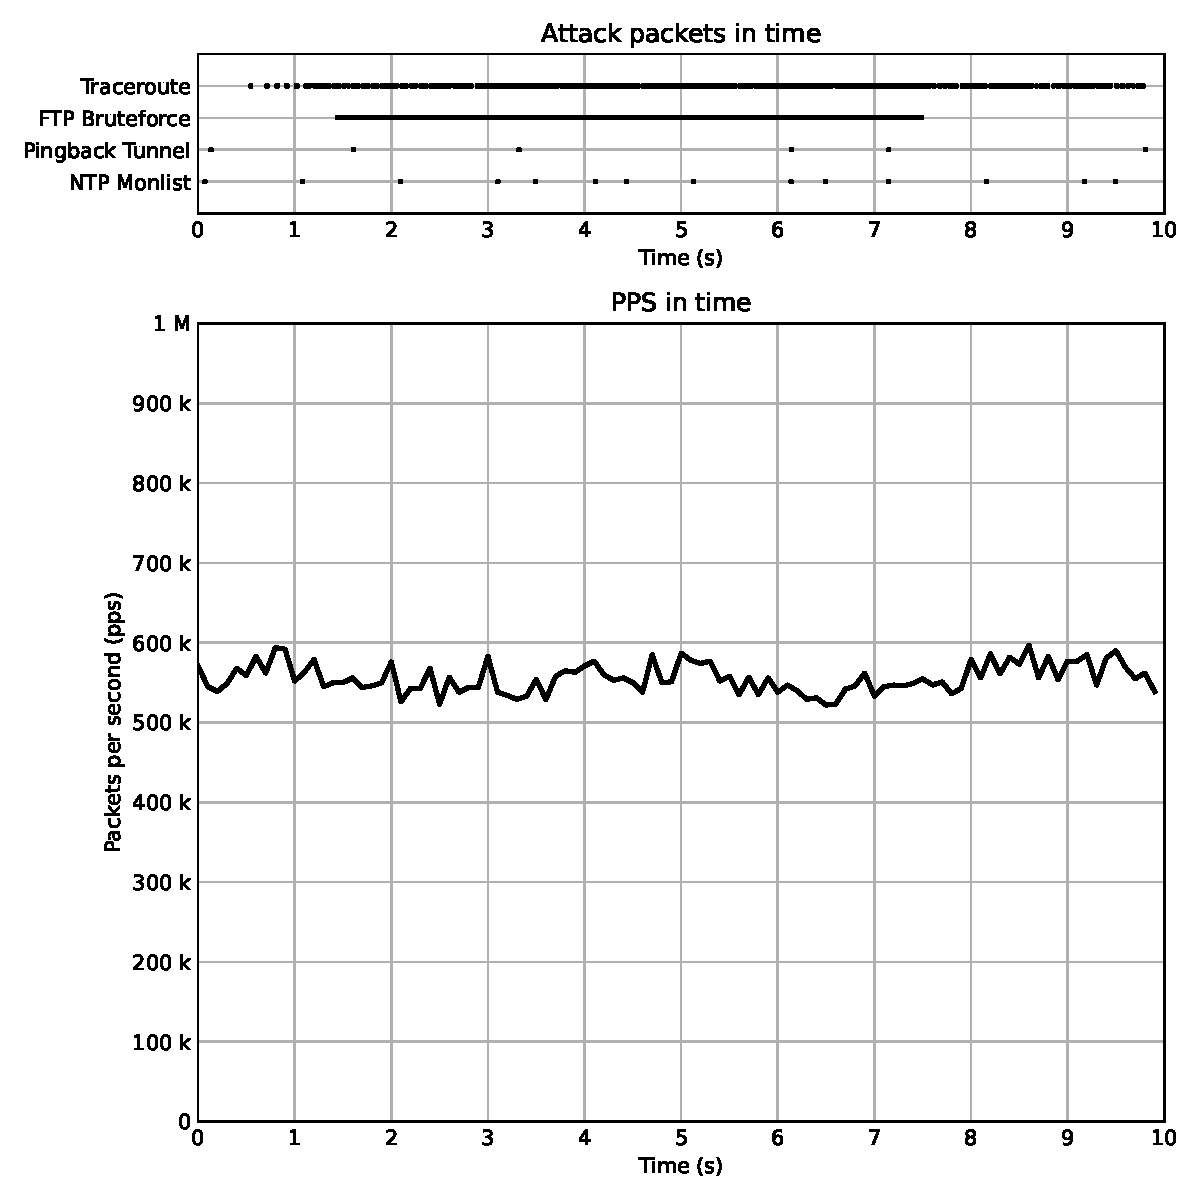
\includegraphics[width=0.7\textwidth]{images/pps_in_time.pdf}  
    \end{center}
    \label{fig:pps_in_time}
    \legend{Source: the author (2022).}
\end{figure}

% Explain the dataset (with plots) + attacks + ferramentas para gerar dataset
% - datasets status: taxa de pico, pps, total size, duration, packets, characteristics...
% - Attacks:
% - FTP Bruteforcing
% - Pingback https://github.com/corelight/pingback
% - Detect traceroute
% - NTP Monlist



\subsection{Experiment setup and methodology}
\label{sec:evaluation:setup}

In this section, we describe the setup of our experiment. The experiment used the same technologies described in \autoref{sec:evaluation:deployment}, relying on network virtualization, P4 emulation to run our switch, and containerization to run Zeek. The objective of our evaluation was to compare the functionality and performance of the Zeek Scripts without RNA, compared with RNA.

Switch emulation does not perform as fast as a real P4 hardware switch, which makes it impossible for us to execute our experiment with a P4 switch in real-time since we only use emulated switches. In this scenario, the emulated switch would become a bottleneck, preventing the traffic from reaching Zeek at the same rate as it enters the P4 pipeline. For this reason, we assess only the performance of the Zeek monitoring system. We assume that a (hardware) programmable forwarding device would be able to execute the program at line rate if the provided program fits the device's memory.

To overcome the performance deficit of emulated P4 switches, we process the combined dataset before running the experiment, effectively creating a second dataset. This second dataset represents a real-world output of a P4-switch, receiving our combined dataset and processing it at line rate. We call this second dataset the \textit{RNA dataset}.

To explain the generation of this second dataset, we use \autoref{fig:rna_dataset_diagram}. The first step is to select from our dataset only the packets that may trigger an Offloader which will eventually generate an mRNA message. With this intermediate trace, we execute our emulated P4 switch, which is now able to process the dataset faster due to the decreased amount of traffic. This results in a dataset with only mRNA messages, the \textit{RNA dataset}. It is also important to note that in all datasets during this process, all packets have their timestamps preserved, and real behavior is emulated.

\begin{figure}[htb]
    \caption{RNA dataset creation diagram}
    \begin{center}
        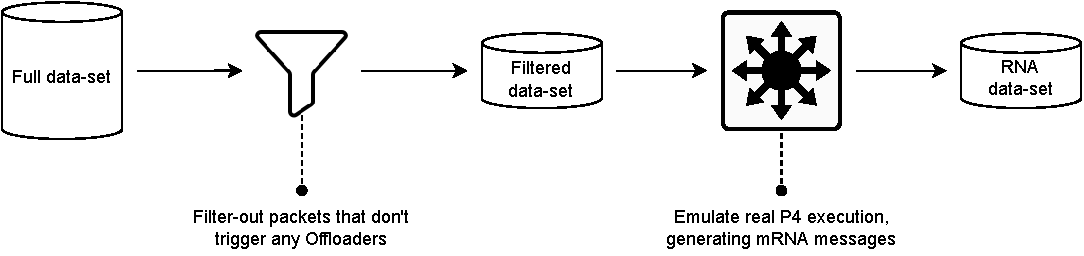
\includegraphics[width=1.0\textwidth]{images/rna_dataset_creation.pdf}  
    \end{center}
    \label{fig:rna_dataset_diagram}
    \legend{Source: the author (2022).}
\end{figure}

Now that we have our two datasets, the \textit{combined dataset}, and the \textit{RNA dataset}, we need to execute Zeek in both scenarios and compare its output and performance. This is done by running Zeek in a Docker container connected to the host computer by a virtual network interface. In this network interface, we replay those two traces, one at a time, and record the memory and CPU usage. Each scenario was executed fifteen times to account for variability. The experiments were executed on a notebook with an Intel Core i9-10885H (\SI{5.3}{GHz}, 8 cores, 16 threads) CPU, \SI{16}{GB} ($2 \times$\SI{8}{GB}) of DDR4 RAM (\SI{3200}{MT/s}), and a \SI{1}{TB} NVMe SSD. While the experiments were executed, in order not to affect the results, no other non-essential services were executed on the computer.

% Methodology?

% \subsection{Methodology}

% Explain results
% - accuracy
%   + script count
% - development cost savings (and less prone to development mistakes)
%   - Show table with multiple combinations of scripts: [1], [2], [3], [4], [1, 2, 3, 4]
% - performance gain
%   - memory, cpu, (execution time/detection time)


\subsection{Results}

In this section, we describe the results of the experiment and functional assessment of our code generation mechanism. We first present the functional results, answering research questions one (RQ1) and two (RQ2). We later present the performance results, answering \textit{RQ3}.

\subsubsection*{Functional results}

To assess whether our proposed mechanism works, we used our prototype and the attacks dataset to compare the output of a Zeek deployment with and without RNA. After executing both setups and comparing the output of Zeek's \textit{notices}, we concluded that our code generation mechanism was able to generate code to successfully offload four different scripts, namely \textit{FTP Bruteforcing}, \textit{Detect traceroute}, \textit{ICMP Pingback}, and \textit{NTP Monlist}. All of these scripts were able to detect, with complete accuracy, all the attacks present in the workload of the experiment, resulting in no difference between the execution with and without RNA in terms of detection.

To answer the second question, we manually inspect the generated code for RNA. Our objective is to check whether our solution is helpful and facilitates the deployment of RNA. \autoref{tab:lines_per_script_count} summarizes the main results obtained. The generated output instance of RNA for offloading our four Zeek Scripts (described above in this section) has $2967$ lines of code. To develop a new Protocol Template, according to \autoref{tab:lines_by_protocol_template}, a median of $40$ lines of code would need to be written, and for a new Offloader Template (\autoref{tab:lines_by_offloader_template}), a median of $224$. This gives developers a big advantage over writing a fully standalone solution since templates are small and easier to maintain than a complete solution. The main advantage leans on the reuse of Protocol and Offloader Templates. Using templates, a network operator is able to deploy RNA without writing a single line of code, only with a command. The automatic code generator identifies the needed events to offload the desired scripts and generates the complete code.


\begin{table}[htb]
    \caption{Lines of Code per Script Count}
    \begin{center}
        \begin{tabular}{|l|r|}
            \hline
            \textbf{Monitoring Script Count} & \multicolumn{1}{l|}{\textbf{Generated Lines Median}} \\ \hline
            1 Monitoring Script              & 2113.5                                             \\ \hline
            2 Monitoring Scripts             & 2421.5                                             \\ \hline
            3 Monitoring Scripts             & 2714.0                                             \\ \hline
            4 Monitoring Scripts             & 2967.0                                             \\ \hline
        \end{tabular}%
    \end{center}
    \label{tab:lines_per_script_count}
    \legend{Source: the author (2022).}
\end{table}

\begin{table}[htb]
    \caption{Lines of code of Protocol Templates}
    \begin{center}
        \begin{tabular}{|l|r|r|r|}
            \hline
            \textbf{Protocol Template} & \multicolumn{1}{l|}{\textbf{Lines of Configuration}} & \multicolumn{1}{l|}{\textbf{Lines of code}} & \multicolumn{1}{l|}{\textbf{Total Lines}} \\ \hline
            Ethernet Protocol          & 13                                                   & 13                                          & 26                                        \\ \hline
            IPv4 Protocol              & 17                                                   & 26                                          & 43                                        \\ \hline
            IPv6 Protocol              & 17                                                   & 20                                          & 37                                        \\ \hline
            ICMP Protocol\footnotemark & 59                                                   & 77                                          & 136                                       \\ \hline
            TCP Protocol               & 22                                                   & 45                                          & 67                                        \\ \hline
            UDP Protocol               & 21                                                   & 10                                          & 31                                        \\ \hline
            \textit{Total}             & \textit{149}                                         & \textit{191}                                & \textit{340}                              \\ \hline
            \textit{Median}            & \textit{19}                                          & \textit{23}                                 & \textit{40}                               \\ \hline
        \end{tabular}%
    \end{center}
    \footnotetext{TODO}
    \label{tab:lines_by_protocol_template}
    \legend{Source: the author (2022).}
\end{table}

\begin{table}[htb]
    \caption{Lines of code of Offloader Templates}
    \begin{center}
        \begin{tabular}{|l|r|r|r|}
            \hline
            \textbf{Offloader Template}        & \multicolumn{1}{l|}{\textbf{Lines of Configuration}} & \multicolumn{1}{l|}{\textbf{Lines of code}} & \multicolumn{1}{l|}{\textbf{Total Lines}} \\ \hline
            NTP Message                        & 27                                                   & 152                                         & 179                                       \\ \hline
            ICMP Echo Message                  & 28                                                   & 157                                         & 185                                       \\ \hline
            ICMP Time Exceeded & 28                                                   & 305                                         & 333                                       \\ \hline
            FTP Request and Reply              & 28                                                   & 235                                         & 263                                       \\ \hline
            \textit{Total}                     & \textit{111}                                         & \textit{849}                                & \textit{960}                              \\ \hline
            \textit{Median}                    & \textit{28}                                          & \textit{196}                                & \textit{224}                              \\ \hline
        \end{tabular}%
    \end{center}
    \label{tab:lines_by_offloader_template}
    \legend{Source: the author (2022).}
\end{table}


% \begin{figure}[htb]
%     \caption{Generated lines per script count}
%     \begin{center}
%         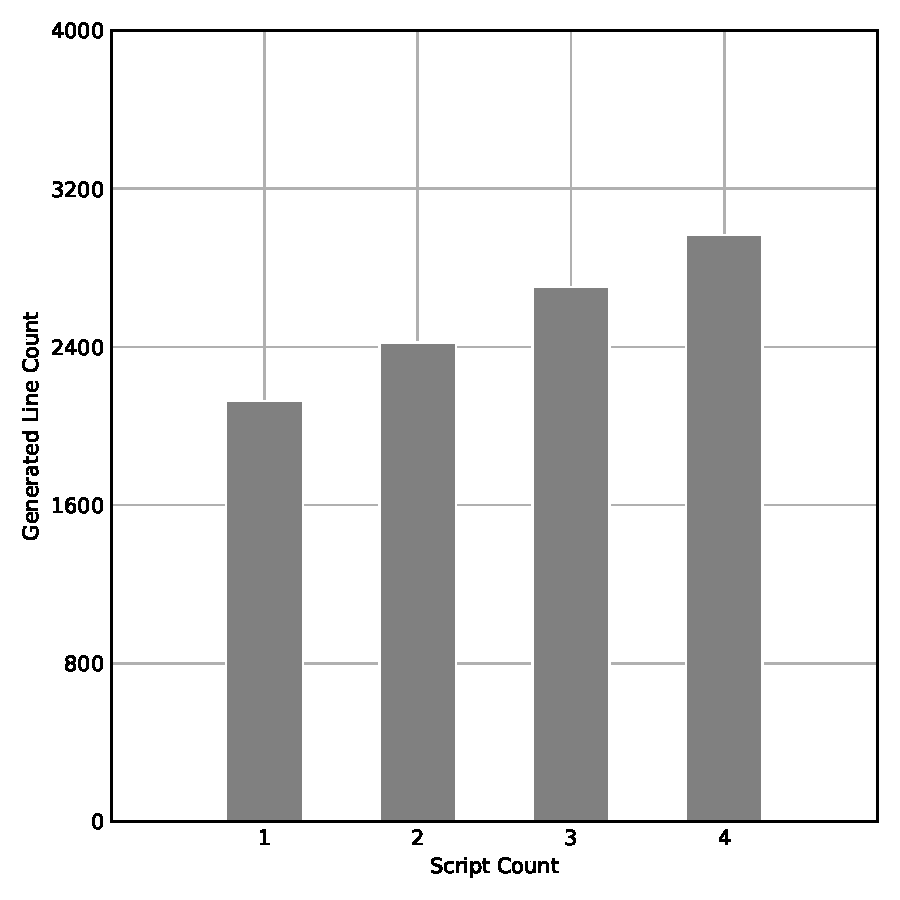
\includegraphics[width=0.7\textwidth]{images/generated_lines.pdf}  
%     \end{center}
%     \label{fig:gen_lines_per_script}
%     \legend{Source: the author (2022).}
% \end{figure}


\subsubsection*{Performance results}

To answer our third research question and assess the performance gain of offloading scripts with RNA, we replayed both of our datasets, the \textit{combined dataset}, and the \textit{RNA dataset}. When replaying the RNA dataset, we enabled our Zeek Plugin, which processed the incoming mRNA messages. This resulted in a significant gain in performance. As Figure \ref{fig:rna_perf} shows, the mean CPU\footnote{Usage of one CPU core. $100\%$ represents usage of a full core, $150\%$ represents usage of one and a half CPU cores.} usage without RNA is $109\%$, and memory usage reaches a maximum of $960.64$ MB by the end of the experiment. With RNA (simulated by using the \textit{RNA dataset}), mean CPU utilization was $1.9\%$ and the maximum memory usage was $235.07$ MB. Additionally, without RNA, a mean of $35.24\%$ of the packets was dropped. The high dropped packet rate resulted in one of the attacks, the \textit{FTP Bruteforce Attack}, not being detected in $93.3\%$ of the iterations executed without RNA. Using our solution, no packets were dropped and all attacks were detected in all executions of the experiment.

In \autoref{fig:rna_perf}, at time \SI{5}{s}, we observe a significant change in the increase of memory and CPU usage. Our hypothesis is that this is the moment internal Zeek buffers are filled, decreasing the rate packets are read, slowing down the increase of memory usage, and increasing the CPU usage. In a real-world scenario, network operators would not allow an IDS to drop packets and would increase the processing power, or implement a sampling strategy. Our intention with this comparison is to contrast the usage of a normal Zeek deployment, compared to our RNA solution, which uses Programmable Data Planes to offload IDS operations. Nevertheless, our results suggest that the observed reduction in CPU usage for the RNA-based setup would allow for the use of a smaller cluster for the given scenario. 

Another important note is that the Dynamic Protocol Detection (DPD), which we presented in \autoref{sec:bg:zeek_ee}, is unable to dynamically detect protocols when RNA is used, potentially resulting in better performance, giving RNA an advantage. This is also one of the assumptions we made to simplify the development of the mechanism.

% Metrics:
% 1. How many scripts we can run (without intervention)
% 2. How many lines were produced per script
%     a. Include copied from the template (maybe create a table with the outline)
% 3. Performance gain in offloading (optional): compare a raw data set vs mRNA messages data set.
%     a. memory, cpu, execution time

\begin{figure}[htb]
    \caption{RNA Performance Evaluation}
    \begin{subfigure}{.5\textwidth}
        \centering
        \vspace{1em}
        \caption{CPU usage by time}
        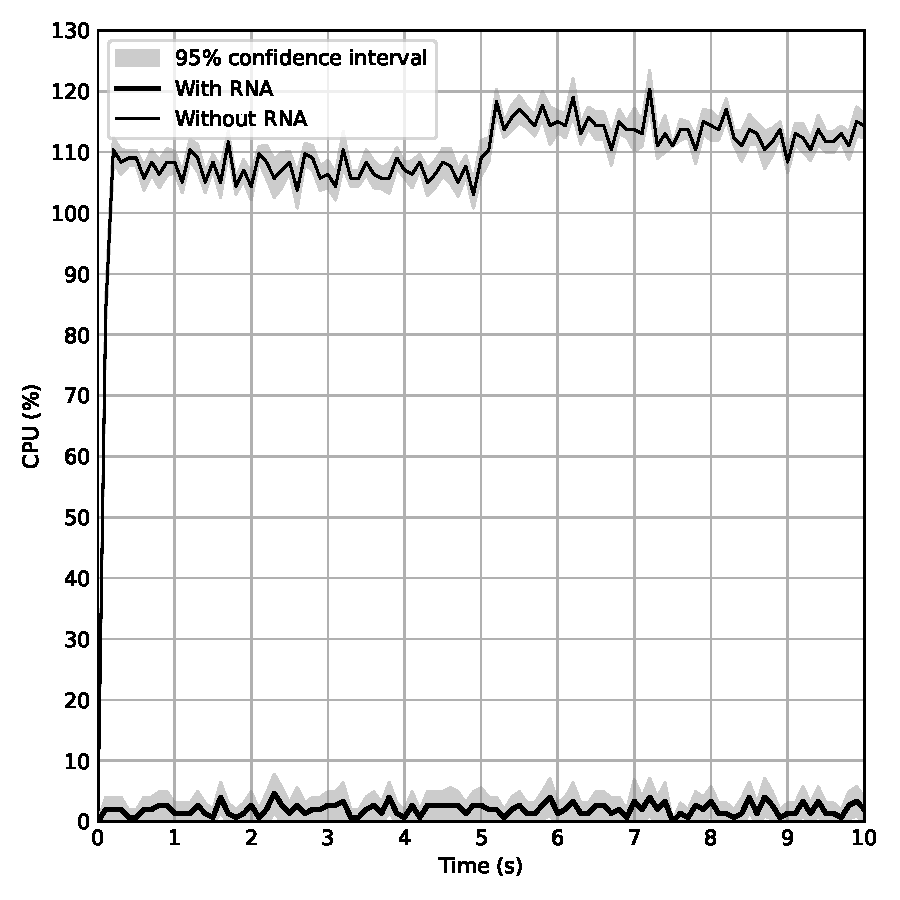
\includegraphics[width=1.0\textwidth]{images/aggregated_cpu_plot.pdf}
        \label{fig:rna_cpu}
    \end{subfigure}%
    \begin{subfigure}{.5\textwidth}
        \centering
        \vspace{1em}
        \caption{Memory usage by time}
        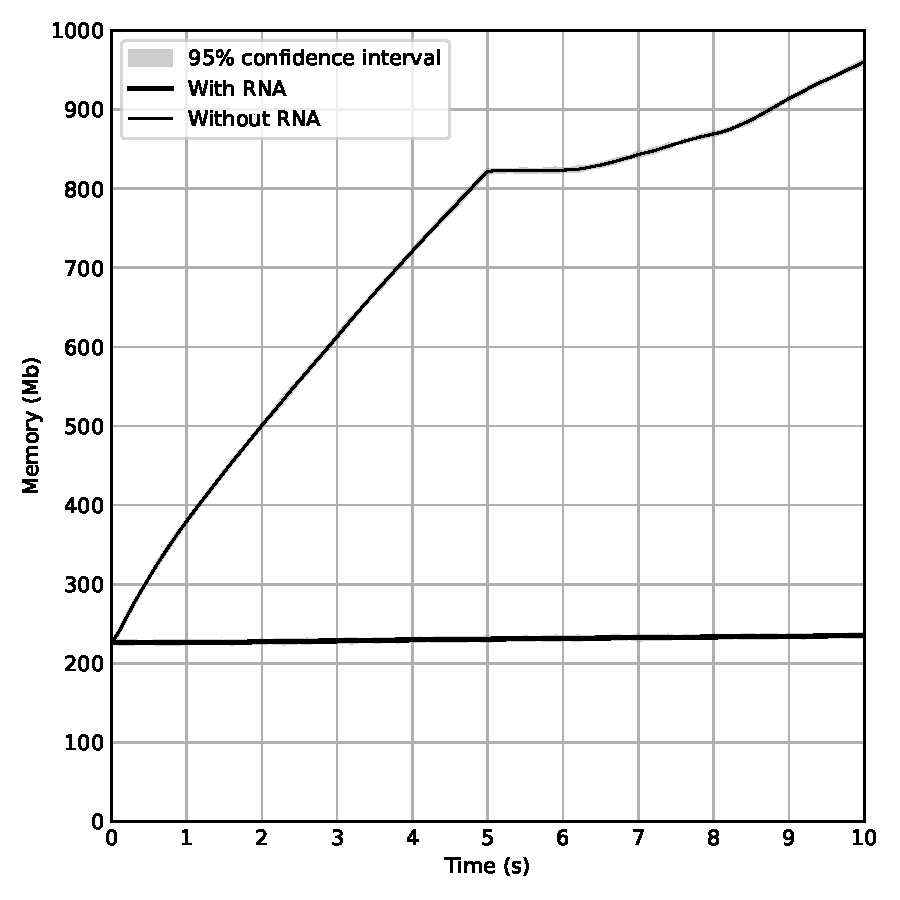
\includegraphics[width=1.0\textwidth]{images/aggregated_memory_plot.pdf}
        \label{fig:rna_mem}
    \end{subfigure}
    \label{fig:rna_perf}
    \legend{Source: the author (2022).}
\end{figure}

% 
% ====================       Pode revisar até aqui :)       ====================
% 
